\section{Background}

\subsection {Aqueous Surface Location}

	In this study we create orientational depth-profiles of \suldiox~and \wat. The reference point used for depth calculations is the location of the water surface. A liquid surface, however, is a dynamic boundary that is neither flat nor stationary. To define a water surface location, several previous studies have used the technique of fitting a lineshape to the averaged density profile of the water, and extracting interfacial shape and location parameters.\cite{Shamay2010,Wick2006c,Chowdhary2006} Hyperbolic tangent functions have been used often, and values for the ``Gibb's dividing surface'' location, and interfacial width have thus been determined.\cite{Matsumoto1988} However, in long simulations the location and shape of the interface changes, and the motion of surface waters alters the interfacial width at any given timestep. Thus, the density profile fitting will capture averaged widths and locations, not instantaneous values. Similarly, the averaged values of location and width will obscure information about any drift or deformations the surface undergoes. In this work we define the surface location by calculating a reference location at each timestep by averaging the positions of the waters contained in the topmost monolayer. This provides us with a consistent and intuitive reference point in the simulations to which we relate our analyses, but does not increase the computational burden.

        The location of the water surface was determined by the averaged positions of a set number of the outer-most waters in the simulated aqueous slabs. The number of waters included in the averaging was decided by taking a few issues into account. First, a visual inspection of the top cross-section of the water slab over several timesteps indicated between 65-75 waters established a full monolayer. Alternatively, assuming a spherical model of water with a radius of 2.2\angs~(the typical length of a bulk-water hydrogen bond), two layers of hexagonally tight-packed spheres would yield a similar number of molecules to the visual inspection. Increasing the number of waters used in calculating the surface location diminishes the effects of the few waters that briefly rise above the surface into the gas phase, stabilizing both the surface position and thickness values. Taking the close-packed model as a maximum number of waters fit into a flat surface, the authors decided to use 70 water molecules for calculating instantaneous water surface locations. 
  
Figure \ref{fig:density-flaw} demonstrates the problem of surface location drift during a simulation. This figure shows the density profile of water and \suldiox~over the course of one of the 10 ns trajectories used in this work. The water density profile and location (dashed line) is produced by averaging the instantaneous density profile at each timestep in the simulation. The water profile was then fit to a $\tanh$ function (black) to extract the position and width parameters of the water surface. The fitted Gibbs dividing surface has a ``90-10'' width of 8.28 $\AA$. A bulge in the gas-phase (left) side of the water density profile is indicative of the drift of the water slab over the course of the trajectory. Thus the calculated location and width from the $\tanh$ line fit are not accurate over long trajectories for defining a stationary reference point. All depth locations in our analyses are calculated relative to the surface location (blue) at the corresponding timestep of the trajectories.

\begin{figure}[h!]
	\begin{center}
		\includegraphics[scale=1.0]{images/density/density-location.png}
		\caption{(A) Density profiles of \wat~(dashed) and \suldiox~(red) from a 10 ns simulation of the neat-water system with a single sulfur dioxide. The \wat~density profile was fit (black) using a hyperbolic tangent function to extract location and width data for the water surface. (B) The location of the outer \wat~monolayer was calculated for each simulation timestep (blue), and the surface location from the density fitting was also determined (dashed). Long simulations of liquid slabs result in drift of the slab location, and the consequent broadening of the water density profile if the surface location is not determined repeatedly throughout the simulation.}
		\label{fig:density-flaw}
	\end{center}
\end{figure}

The new procedure described above for finding the outer monolayer location was implemented, and the distribution of that location is also plotted in figure \ref{fig:density-flaw} (blue). It is apparent from the surface location distribution that the water slab drifts over the 10 ns, spanning approx. 12 $\AA$. However, the maximum standard deviation of the positions of the waters comprising the surface layer at each timestep is only 1.85 $\AA$. 

  %Taking one of the simulations of the neat-water slabs, a series of calculations were performed to find the averaged positions and the standard deviations of varying numbers of the topmost waters. It was found that using 70 waters produced a standard deviation of the water positions corresponding to a width of 3.2\angs. as reported by Baer et al.when fitting the density profile with a hyperbolic tangent lineshape. To match the interfacial width of Baer using the standard deviation of our simulations, 70 water molecules would have to be included in the top monolayer. Thus, the calculations and analyses presented in this work incorporate 70 water molecules when calculating the surface location.


\subsection{Analysis of Molecular Orientation}

	The simulated systems were analyzed to characterize the orientation of \wat~and \suldiox~in various environments above, within, and below the aqueous surface region. In order to better understand the chemistry occurring during the \suldiox~adsorption process, the molecular orientation of both the \wat~and \suldiox~must be understood.  The two molecules studied are similarly shaped with a C2$_v$ axis along their bisectors, and a molecular plane defined by three atoms. A body-fixed frame is defined for both \wat~and \suldiox~as shown in figure \ref{fig:molecular-frame}. In each analysis a space-fixed reference axis is used that corresponds to the long axis of the system's periodic cell normal to the plane of the water surface. The orientational analyses presented herein focus on two angles used to define molecular orientation. The molecular orientation angles $\theta$ and $\phi$ are determined from a set reference axis as shown in figure \ref{fig:water-angles}a.
	
	The ``tilt'' angle, $\theta$, defines the angle formed between the molecular bisector vector (the molecular z-axis, pointing from the central atom in the direction of the other two atoms) and the positive system reference axis. Thus the value of $\theta$ falls within a range of $[0,\pi]$. An angle of $\cos(\theta)=1$ indicates a molecule with its bisector aligned with the reference axis, while $\cos(\theta)=-1$ results from an anti-aligned configuration. Sample representations of different values of $\cos(\theta)$ are shown in figure \ref{fig:water-angles}b.
	
	A second angle, $\phi$, defines the molecular ``twist'' for certain configurations of the molecule. $\phi$ is the angle formed between the vector normal to the plane of the molecule (molecular y-axis) and the system reference axis. The values of $\phi$ fall in the interval $[0,\frac{\pi}{2}]$ because of the symmetry of \wat~and \suldiox~molecules with respect to twist about their bisector axes. For values of $\cos(\theta) \approx 0$, $\phi$ provides additional information about whether the molecular orientation is ``flat'' to the surface (e.g. the plane of the molecule is aligned with the plane of the surface), or if it is perpendicular. The values of $\cos(\phi)$ for different molecular orientations are shown in figure \ref{fig:water-angles}c. %However, the symmetry of the \wat~and \suldiox~molecules create equivalence between the two H, or O, atoms (in the \wat~or\suldiox, respectively). $\phi=-\pi$ is equivalent to $\phi=\pi$, and both situations are equivalent to $\phi=0$. Because $\phi=-\phi$, the value is reported within the range of $[0,\frac \pi 2]$. 
	However, values of $\cos(\theta)$ close to 1 or -1 result in an isotropic distribution in $\cos(\phi)$ because of the symmetry of the plane of the surface in directions perpendicular to the reference axis.

%	The two molecules studied, \wat~and \suldiox, and similarly shaped with a C2$_v$ axis along their bisectors, and a molecular plane is defined by their three atoms. The orientational analyses presented herein focus on two angles used to define the molecular orientation in space. In each analysis a reference axis is used to define molecular angles, and is the z-axis unless otherwise specified. A ``tilt'' angle, $\theta$, defines the angle formed between a vector (generally the bisector vector pointing from the central atom in the direction of the other two atoms) and the positive reference axis. Thus the value of $\theta$ falls within a range of $[0,\pi]$. A second angle, $\phi$, defines the molecular ``twist'' around the reference axis. $\phi$ is formed between the projection of a vector onto the x-y reference plane, and the x-axis. $\phi$ is thus defined relative to the x-axis, and its values are in the interval $[-\pi,\pi]$. However, because of the symmetry of the \wat~and \suldiox~molecules and the equivalence of the two H or O atoms (in the \wat~or\suldiox, respectively), $\phi=-\pi$ is equivalent to $\phi=\pi$, and both situations are equivalent to $\phi=0$. Because $\phi=-\phi$, the value is reported within the range of $[0,\frac \pi 2]$. Figure \ref{fig:spherical-angle} shows the angle definitions using the z-axis as the reference axis.

\begin{figure}[h!]
	\begin{center}
		\includegraphics[scale=1.0]{images/angle-cartoons/molecularframesmall.png}
		\caption{Molecular body-fixed axes are defined with the x-z plane formed by the three atoms, and the z-axis aligned to the molecular bisector. The y-axis is normal to the molecular plane, and one of the bonds points in the positive x direction.}
		\label{fig:molecular-frame}
	\end{center}
\end{figure}

\begin{figure}[h!]
	\begin{center}
		
\includegraphics[scale=1.0]{images/angle-cartoons/molecular-angles.png}
		\caption{(A) The definition of the angles $\theta$ and $\phi$ used to define molecular orientation of \suldiox~and \wat~relative to a reference axis. (B) $\theta$ is the value of the ``tilt'' of the molecular bisector from the reference axis, with $\cos(\theta)$ values ranging from -1 to +1 indicating different bisector orientations. (C) $\phi$ is the ``twist'' angle formed between the vector normal to the molecular plane (the body-fixed y-axis) and the reference axis. For values of $\cos(\theta) \approx 0$, $\phi$ shows how flat the molecule is relative to the interfacial plane.}
		\label{fig:water-angles}
	\end{center}
\end{figure}

%\subsection{Hydrate Complex Analysis}

%During the adsorption process of a gaseous \suldiox~moving in towards a water surface hydrate complexes are formed as the waters bind to the molecule. Computationally, there are various methods to determine hydrate complex formation. The most simple metric is to count the number of hydrogen bonds formed from the \suldiox~to neighboring molecules. This method can be furthered extended to also include the strength of those bonding interactions by additionally reporting the bondlengths to the hydrogen bonding partners. Longer bondlengths are typical of weaker bonds, and this method is used in this work to identify the bonding environment of the \suldiox~during solvation.

%A simple count of hydrogen bonds is telling of the interactions and environments of an adsorbing \suldiox. However, a more sophisticated analysis is needed to fully characterize the geometry of any complexes that form. In this work a graph theoretical method has been used to identify hydrate complexes that form cyclic structures in addition to those that form more simple hydrogen bonding geometries. Previously published works have detailed graph theory for use in molecular systems, and have used graph theoretical methods to describe ice and water clusters, structural energies, as well as in the study of relationships in biological systems.\cite{Huber2007,Shi2005,Radhakrishnan1991,Anick2002} As such, we will not present here a review of the basic graph theoretical details that are well documented in the referenced works. As shown in figure \ref{fig:so2-complex-graph}, the atoms of a \suldiox~and its nearest neighbors are represented as a set of verrtices, with the covalent and hydrogen bonds between them forming the edges of a graph.

%We present here a technique for determining bonding cycles in a hydrate complex, but this technique is general enough to be applied to any graph representation of simple molecular systems. The first step in the determination of cycles is translating the atoms (vertices) and bonds (edges) to a graph. Figure \ref{fig:so2-complex-graph} shows the procedure visually, where here the root vertex of the graph is the \suldiox-sulfur, and each atom is numbered by the distance, in atoms, to the root vertex. We use only the closest neighboring water molecules that may take part in a cyclic complex in building the graph. After forming the graph, a breadth-first search (BFS) is performed starting at the root vertex.\cite{Knuth1997} The BFS algorithm uses a coloring technique where all unexamined vertices are colored white, queued vertices are gray, and examined vertices are black. During the BFS, encountering a gray vertex as a target of an adjacent edge during examination indicates that a cycle has been found in the graph. At each vertex dequeue for examination, the parent of every vertex is recorded such that the lineage from gray target to root vertex can be reconstructed to determine the participating atoms in the cycle.

%\begin{figure}[h!]
%\begin{center}
%\includegraphics[scale=1.0]{images/Cycles/so2complexfigure.png}
%\caption{A \suldiox~and its nearest neighbors are represented as a graph of vertices and edges. The bonds are all given equal weights and the graph is undirected. The numbering shows the relative distance from any atom to the root node (\suldiox-sulfur 1), and also enumerates the iteration through the BFS process at which the atom is discovered. A BFS on this graph would result in discovering the doubly-bound hydrogen (5) as a gray target, and the gray source would be either of the connected oxygens (4). At each iteration the predecessor in the BFS is recorded in order to reconstruct the connectivity of the cycle. This cycle is composed of 8 atoms, and 3 molecules}
%\label{fig:so2-complex-graph}
%\end{center}
%\end{figure}
